\chapter{Collisional transport}
\label{chap:TransportCollisionnel}


This theory was developed in the 60-70s. First it has obtained results on electron particle and energy transport, then on impurities. The object of this section is to summarise the mst important results of the theory, with a few calculations to illustrate the physics at play.



		\section{Motivations}
		\label{sec:TransportCollisionnelMotivation}

Up to now, the transport properties in tokamak plasmas have been demonstrated with a minimum number of hypotheses and very general evolution equations. Now we are going to be concerned with the first theory which has attempted to describe the nature of transport and the physical quantities which play a role in it. This theory, often called 'neoclassical theory', aims at calculating the various heat and particle fluxes due to collisions between charged particles.

first let us consider that these collisions give rise only to diffusion of particles in the plasma. an estimate of the resulting diffusion coefficient can be obtained by assuming that the (radial) displacement of a charged particle due to a collision is of the oredr of the Larmor radius. Let us denote $\nu_c$ the collision frequency of this particle. Its diffusion coefficient can be written:

\[
		\chi = \rho_L^2 \nu_c
\]

The particle lifetime in the plasma is then of the order of:
\[
\tau \simeq \frac{a^2}{\chi} = \frac{a^2}{\rho_L^2}\frac{1}{\nu_c}
\]

With reasonable values $a = 1$ m, $\rho_L = 10^{-3}$ m and $\nu_c = 250$ s$^{-1}$, we find $\tau \simeq 4\times 10^3$ s which is obviously much longer than any measured value in a tokamak. In the simplistic configuration assumed here (no force is applied ot the charged particles) the (vertical) curvature drift is responsible for a vertical electric field which causes an electric drift directed outward (away from the plasma magnetic axis). This drift drives the particles out of the plasma in less than 1 ms. This is why the tokamak magnetic configuration has been chosen: the curvature drift forces the particles to remain in the vicinity of their magnetic surface and thus reduced the electric drift effet. 

Let us now consider a situation closer to the tokamak one: cylindrical geoemtry, a magnetic field $\vec{B}$ and an elecrtric field $\vec{E}$ imposed from outside. The generalised Ohm's law can be expressed as:
\begin{equation}
	\vec{E} + \vec{v}\times\vec{B} = \eta\vec{j} + \frac{1}{en}\left( \vec{j}\times\vec{B} - \vec{\nabla}p \right)
	\label{LoidOhm}
\end{equation}
where $\eta$ is the plasma resistivite.
In addition, the pressure balance equation is:
\[
	\vec{j}\times\vec{B} = \vec{\nabla}p
\]
The vector multiplication of equation \ref{LoidOhm} by $\vec{B}$ and the use of the pressure balance equation allow to obtain:
\[
	\vec{E}\times\vec{B} - \vec{v}_{perp}B^2 = \eta\vec{\nabla}p
\]
or equivalently:
\[
		\vec{v}_{perp} = -\frac{\eta}{B^2}\vec{\nabla}p + \frac{\vec{E}\times\vec{B}}{B^2}
\]
 
The first term of the perpendicular velocity is due to collisions (as indicated by the $\nabla p$ term), the second one being the electric drift.

The particle flux associated with collisions is thus:
\[
	\vec{\Gamma}_{perp}^{coll} = nv_{perp}^{coll} = -\frac{\eta n}{B^2}\vec{\nabla} p
\]
If the temperature is uniform, we have $\vec{\nabla}p = T\vec{\nabla}n$, which gives:
\[
\vec{\Gamma}_{perp}^{coll} = -\frac{\eta \beta}{2\mu_0}\vec{\nabla}n
\]
where $\beta$ is the kinetic to magnetic pressure ratio:
\[
	\beta = \frac{nT}{B^2/2\mu_0}
\]
We cna then deduce the so-called \textit{classical} diffusion coefficient:
\[
		D_{cl} = \frac{\eta\beta}{2\mu_0}
\]



		
		\section{Collision frequency}
		\label{sub:FrequenceDeCollision}
			
			
				\subsection{Debye length}
				\label{subsub:LongueurDeDebye}


Due to the long range of the electromagnetic interaction, in principle the Coulomb interactions occur between any charged particle pair, whatever the distance between the two particles. Actually, beyond a certain distance (called \textit{Debye length}), the particles do not see each other because of a screening effect. The Debye length has the following expression:
\begin{equation}
		\lambda_D = \sqrt{\frac{\epsilon_0 kT}{n e^2}}
		\label{Debye}
\end{equation}
where $T$ and $n$ are the plasma temperature and density respectively and $e$ is the particle charge. It is assumed here thatthe plasma contains only one particle type. It is still valid if the plasma impurity content is not too high.

Each particle is sensitive to the electrostatic potential due to all the surrounding charges within a distance less than $\lambda_D$. This part of the space is referred to as the Debye sphere, volume $4/3(\pi\lambda_D^3)$, centered at the considered particle and moving with it. We will consider that the screening effect is perfect, i.e. that there are no Coulomb interactions of a particle with those outside this sphere.

The movement of each particle is influenced at every time by the potential created by its neighbours inside the Deby sphere, and these neighbours are themselves subject to the same rule. As a consequence, there are weak and fast variations of the electrostatic potential at each point of the plasma. These fluctuations are at the origin of electrostatic turbulence, qui is not taken into account in the neoclassical theory because it requires specific developments. Transport due to electrostatic turbulence is described in Chapter \ref{chap:TransportTurbulent}.


				\subsection{Landau length}
				\label{DistanceDeLandau}


Due to electrostatic repulsion, there is a lower bound for the distance between two charged particle with same sign charges. This limit is called the \textit{Landau length}. It can be easily calculated with the help of the energy conservation law in the frame of one of the particles (particle 1 in the following). The energy conservation of particle 2 writes:

\[
			E_2 = \mbox{constante, avec } E_2 = E_{p_2} + E_{c_2},
\]
$E_{p_2}$ and $E_{c_2}$ are the potential energy and kinetic energy of particle 2. At infinity, $E_{p_2} = 0$, which implies that $E_2 = E_{c_2}^\infty = kT$. Ath minimal distance $\lambda_L$, we have $E_{c_2} = 0$ and hence $E_{p_2} = kT$. Since the potential energy is due to the electrostatic potential, we have $E_{p_2} = e_1 e_2 / 4\pi\epsilon_0\lambda_L$. We can then deduce the Landau length:
\begin{equation}
		\lambda_L = \frac{e_1 e_2}{4\pi\epsilon_0 kT}.
		\label{Landau}
\end{equation}

In a tokamak plasma, the typical temperatures are around 100 eV at the edge and 10 keV in the centre. The Landau length for the plasma ions thus range from $10^{-11}$~m to $10^{-13}$~m: the fusion reactions, due to the strong interaction (range $10^{-15}$~m), occur mainly thanks to the tunnel effect.


						
				\subsection{Calculation of the collision frequency}
				\label{subsub:CalculDeLaFréquenceDeCollision}

A 'collision' between two charged particles in a plasma cannot be described as that of two billiard balls. Therre is neither impact nor contact but onyl deflection. The problem is generally treated under the name of \textit{Rutherford scattering} and the result is the deflection angle of the projectile as a function of its initial trajectory distance to the target. This distance is called the impact paramtere and will be dented $b$ in the following. In a tokamak plasma a particle is deflected more or less permanently by a multitude of interactions with its neighbours. Most of the time, these interactions occur at fairly large impact parameters and thus cause small deflections. Moreover, as a particle moves with its Debye sphere, no binary collision is complete. This is thus far from the academic Rutherford scattering case. Even the definition of a collision becomes a problem. What is the limit deflection angle (or impact parameter) above (below) which we consider a collision has occurred?

This question is answered by defining a collision by its effect. The trajectory modification corresponding to what will be called a collision is fixed arbitrarily. One of the possible criteria is that the total deflection angle resulting from a series of distant binary collisions be 90°. Another criterion is that the variation of the velocity module of a particle $\Delta v = \sum{||\delta \vec{v}||}$ be equal to $v$. Our choice for the calculation to follow concerns the velocity square. A collision will be saisd to occur when:
\[
		\Delta v^2 = \sum{(\delta v)^2} = v^2.
\]

Let us go back to the elementary case of a binary collision between a projectile (moving particle, subscript 1) and a target (unmoving particle, subscript 2). The second Newton's law allows to write the variation rate of the moving particle speed as a function of its distance $r_{12}$ to the target particle:
\[
		\frac{dv_1}{dt} = \frac{e_1 e_2}{4\pi\epsilon_0 m_1 r_{12}^2}
\]
Most of the binary interaction occur at large impact parameter. They cause alomost no deflection dunring the approach and escape phases. Their effect will be coonsidered only when particle 1 is in the vicinity of particle 2, i.e. when $r_{12} \simeq b$. This phase lasts only for approximately $\delta t \simeq b/v_1$. The speed change due to a binary collision is thus:
\[
		\delta v_1 \simeq \frac{e_1 e_2}{4\pi\epsilon_0 m_1 v_1 b}.
\]
Note that it decreases when the speed is increased. This trend will appear again in the collision frequency.

We are now going to calculate the variation of the square module of the velocity over a longer time interval  $\Delta t$. During $\Delta t$ and for an impact parameter between $b$ and $b+db$, particle 1 will be interacting with $n_2 \times 2\pi b.db.v_1.\Delta t$ particles of population 2. The speed change associated with impact parameter $b$ is thus:
\[
		\Delta (v_1^2)_b = \sum{(\delta v_1)^2} = \left( \frac{e_1 e_2}{4\pi\epsilon_0 m_1 v_1 b} \right)^2 \times 2\pi b.db\times n_2 v_1 \Delta t
\]
and, for all possible values of the impact parameter:
\begin{eqnarray}
		\Delta (v_1^2) 	&	=	&	\int_{b_{min}}^{b_{max}} \Delta (v_1^2)_b \nonumber\\
										& = &	\int_{b_{min}}^{b_{max}} \left( \frac{e_1 e_2}{4\pi\epsilon_0 m_1 v_1 b} \right)^2 \times 2\pi b.db\times n_2 v_1 \Delta t	\nonumber	\\
										& \simeq &	\frac{e_1^2 e_2^2}{\left( 4\pi\epsilon_0 \right)^2 m_1^2 v_1}.n_2\ln{\frac{b_{max}}{b_{min}}}\Delta t
\end{eqnarray}
(we have put aside a factor $2\pi$ in order to retrieve the usual expression of the collision frequency). The minimum impact parameter $b_{min}$ is that below which no collision occurs. In practice this bound can be set to the Landau length, which strictly speaking is not an impact parameter (it is the minimal distance between two particles in a front collision, i.e. $b = 0$) but is small compared to the average distance between particles ($1/n^3$).

The maximum impact parameter $b_{max}$ is that beyond which there is no interaction . It is the definition of the Debye length, hence $b_{max} = \lambda_D$. The term $\ln{\lambda_D/\lambda_L}$ is often written $\ln \Lambda$. It is called the Coulomb logarithm. Whatever the experimental situation it is always in the range 10 to 20 (more often 15 to 18).

The collision frequency definition we have chosen means that $\Delta v_1^2 = v_1^2$ when $\Delta t = 1/\nu_{12}$, $\nu_{12}$ being the collision frequency of a particle of type 1 in a population of type 2. It can be easily deduced that: 
\begin{equation}
		\nu_{12} = \frac{e_1^2 e_2^2}{\left( 4\pi\epsilon_0 \right)^2 m_1^2 v_1^3}.n_2\ln{\Lambda}
\end{equation}

Let us recall that this expression is valid in the case of a moving particle of type 1 and an unmoving population of type 2. Therefore it can be applied to calculate the collision frequency of an electron (light and thus fast) on a population of ions (heavy and thus almost at rest):
\[
		\nu_{ei} = \ln{\Lambda} \frac{e^4}{\left( 4\pi\epsilon_0 \right)^2 \sqrt{m_e} kT_e^{3/2}}.n_i
\]

It is not exactly applicable to the collision frequency of electrons onto themselves or of ions onto themselves but still it is often used with a correction factor $1/\sqrt{2}$:
\[
		\nu_{ee} = \ln{\Lambda} \frac{e^4}{\sqrt{2}\left( 4\pi\epsilon_0 \right)^2 \sqrt{m_e} kT_e^{3/2}}.n_e = \frac{1}{\sqrt{2}} \frac{n_e}{n_i}\nu_{ei}
\]
and
\[
		\nu_{ii} = \ln{\Lambda} \frac{e^4}{\sqrt{2}\left( 4\pi\epsilon_0 \right)^2 \sqrt{m_i} kT_i^{3/2}}.n_i = \sqrt{\frac{m_e}{m_i}} \left( \frac{T_e}{T_i} \right)^{3/2} \frac{n_i}{n_e}\nu_{ee}
\]

To calculate $\nu_{ie}$, let us work in the general situation i.e. without any assumption on the particle mass or speed. The momentum variation of particle 1 in the population 2 is:
\[
\frac{d\vec{p}_1}{dt} = m_1 \nu_{12} \left( \vec{v}_1 - \vec{v}_2 \right)
\]
La variation de la quantité de mouvement totale de la population 1 est donc:
\[
\frac{d\vec{P}_1}{dt} = n_1 m_1 \nu_{12} \left( \vec{V}_1 - \vec{V}_2 \right)
\]
where $\vec{V}_1$ and $\vec{V}_2$ are the average speeds of the populations. This variation corresponds to the friction force $\vec{F}_{21}$ exerted by population 2 on population 1. Following the third Newton's law (the action-reaction principle) population 1 exerts a force of same intensity and opposite direction on population 2: $\vec{F}_{12} = - \vec{F}_{21}$, which we use to find the relation between $\nu_{12}$ et $\nu_{21}$:
\[
		n_1 m_1 \nu_{12} = n_2 m_2 \nu_{21}
\]
We can deduce the collision frequency of ions onto electrons:
\[
		\nu_{ie} = \ln{\Lambda} \frac{e^4}{\sqrt{2}\left( 4\pi\epsilon_0 \right)^2 m_i^2 \left(\frac{kT_e}{2m_e} \right)^{3/2}}.n_e = \left( \frac{m_e}{m_i} \right)^2 \nu_{ee}
\]
With the assumptions $n_e = n_i$ and $T_e = T_i$, we thus have the ordering:
\[
		\nu_{ie} << \nu_{ii} << \nu_{ee} \simeq \nu_{ei}
\]

We can see that the ion thermal equilibration time is shorter than the electron-ion energy equipartition time. It could be demonstrated also that the collision frequency of impurities on ions is large enough for the two populations to be always at the same temperature.






										
		\section{Collisional regimes}
		\label{sub:RegimesCollisionnels}
				
On the basis of simple consideration on the propoerties of charged particle trajectories in tokamaks, it can be demonstrated that the diffusion coefficient takes different forms according to the range in which the collision frequency lies. This is what we are going to show now.


-------------------------------------------------

				
				\subsection{Reminder on trajectories}
				\label{subsub:RappelsTrajectoires}
						
Most of this reminder concerns trapped particle trajectories:
\begin{itemize}
		\item Trapping condition:	$\left( v_\| / v_{\bot} \right)_{\theta = 0} \leq \sqrt{2\epsilon}$
		\item Banana orbit width:	$\delta_b \simeq \frac{mv_\phi}{eB_\theta} \simeq \frac{2q}{\sqrt{\epsilon}}\rho_L$
		\item Detrapping frequency:	$\nu_{eff} = \nu_c/2\epsilon$
		\item Bounce frequency:	$\nu_b = v_\| / 2\pi q R \simeq v_{th}\sqrt{\epsilon} / 2\pi q R$
		\item Fraction of trapped particles: $f_p = \sqrt{2\epsilon}$
\end{itemize}
The inverse aspect ratio is denoted $\epsilon = r/R$ and the collision frequency $\nu_c$.

We define also the transit time of passing particles as the time necessary for them to go from the low field side midplane to the high field side midplane (or the opposite way): $\tau_\| = \pi q R / v_{th}$. To this time we associate the transit length $L_\| = \pi q R$ and the transit frequency $\nu_\| = 1/\tau_\|$.
						
						
				\subsection{Strongly collisional regime: Pfirsch-Schlüter}
				\label{RegimePfirschSchluter}
	
In this regime the mean free path of passing particles is shorter than the transit length, which writes:
\[
		\nu_c >> \frac{v_\|}{L_\|} \simeq \frac{v_{th}}{\pi qR}
\]
assuming $v_\| \simeq v_{th}$. In the random walk process already discussed, we will asume now that the elementary deviation due to a collision is of the order of the displacement due to the vertical drift during time $\tau_\|$:
\[
		\Delta = v_d \tau_\| = \frac{\rho_L}{R}v_{th}\tau_\| = \pi q \rho_L
\]
The diffusion coefficient in this case is thus:
\[
		D_{PS} = \Delta^2 \nu_c = \pi^2 q^2 \rho_L^2 \nu_c
\]
It is proportional to the collision frequency.



				\subsection{Weakly collisional regime: banana}
				\label{RegimeBanane}


We consider now a situation in which the detrapping frequency is so small that trapped particles can travel several time their orbit before being detrapped:
\[
		\nu_{eff} << \nu_b \Longleftrightarrow \nu_c << \frac{v_{th}}{\pi q R}\epsilon^{3/2}
\]
It is easily checked that in this case the collisions between passing particles are extremely rare. On the cotrary, trapped particles can have several collisions on their orbit before they are detrapped. Each collision modifies slightly their orbit and when detrapped they can leave their orbit at a radius different from that at which they were trapped. They are thus the main contributors to transport. 

The radial deviation of a particle between its trapping time and its detrapping time is of the order of the orbit width. Taking into account the fraction of trapped particles, the associated diffusion coefficient is thus:
\[
		D_B = f_p \Delta^2 \nu_{eff} = \frac{q^2 \rho_L^2}{\epsilon^{3/2}}\nu_c
\] 

	
	
				\subsection{Intermediate regime: plateau}
				\label{RegimePlateau}

\hspace{1cm} Between the two extreme regimes, only a part of the trapped particles will have many collisions before being detrapped (passing particles are still very weakly collisional). This part is of the order of $\nu_b/\nu_{eff}$. The diffusion coefficient in this regime is thus:
\[
		D_P = \frac{\nu_b}{nu_{eff}}D_B = \frac{q}{R}\rho_L^2 v_{th}
\]

The existence of three collisionality regimes is illustrated in Fig. \ref{fig:Regimes_collisionnels} for typical values of Tore Supra and ITER presented in Table \ref{tab:Regimes_collisionnels}.


\begin{figure}[htbp]
	\centering
		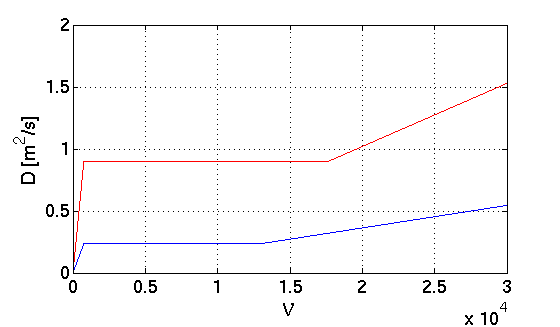
\includegraphics[width=0.70\textwidth]{Fig_Regimes_collisionnels.png}
	\caption{Dependence of the neoclassical diffusion coefficients as a function of collisionality. Electrons are always in the banana regime($\nu_e* \simeq 0,2$ in Tore Supra et 0,06 in ITER),ions are between banana regime and plateau regime, impurities are in the plateau (light impurities or very hot plasmas) or Pfirsch-Schlüter (heavy impurities or colder, thinner plasmas) regime.}
	\label{fig:Regimes_collisionnels}
\end{figure}
\begin{table}[htbp]
	\centering
		\begin{tabular}{|c|c|c|}
			\hline
			Grandeur											&		Tore Supra				&		\textit{ITER}	\\
			\hline
			B (T)													&				3,8						&		8							\\
			R	(m)													&				2,35					&		6							\\
			r (m)													&				0,35					&		0,7						\\
			q															&				2							&				2					\\
			kT (keV)											&				1							&				10				\\
			mc$^2$ (keV) =	m$_D c^2$			&	$2\times 10^6$			&	$2\times 10^6$	\\
			e	(C)													&		1,6.10$^{-19}$ 		&	1,6.10$^{-19}$	\\
			\hline
			$v_{th} = \sqrt{kT/m}$ (m/s)	&		$2.10^5$m/s				&	$6,7.10^5$ 			\\
			$\rho_L = m_D v_{th,D} /eB$ (m)	&			1,2.10$^{-3}$		&		2.10$^{-3}$		\\
			$\epsilon$										&				0,15					&			0,12				\\
			\hline
		\end{tabular}
	\caption{Parameter values used to draw the curves of Fig. \ref{fig:Regimes_collisionnels}}
	\label{tab:Regimes_collisionnels}
\end{table}


				\subsection{Collisionality}
				\label{Collisionnalite}

The numerical value of the collision frequency is not enough to know in which collisional regime a particle is, unless the physical and geometrical quantities of the plasma under study are known. For a more universal criterion, we define a normalised collsion frequency called \textit{collisionnality}:
\[
		\nu* = \frac{\pi q R}{v_{th}\epsilon^{3/2}}\nu_c
\]

The collisionality domains are bound by values $\nu* = 1$ (banana-plateau boundary) et $\nu* = \epsilon^{-3/2}$ (plateau-Pfirsch-Schlüter boundary). A typical value for deuterium in ITER is $\nu_D* \simeq 0,05$. Among the present day machines, only the largest ones can reach this collisionality range, and only for the high temperature scenarios.

On Fig. \ref{fig:nustar_D_Ni_39601} typical collisonality profiles are shown  in Tore Supra for the main ions species (deuterium) and nickel, taking into account the presence of intrinsic impurity species (carbon and helium).
\begin{figure}[htbp]
	\centering
		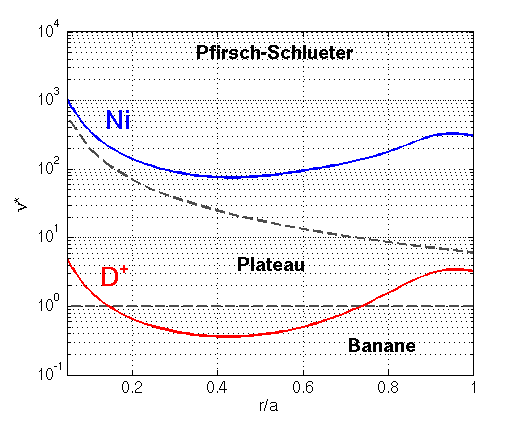
\includegraphics[width=0.70\textwidth]{Fig_nustar_D_Ni_39601.png}
	\caption{Radial profiles of collisionality for deuterium and nickel in a tore supra plasma. The dashed curves represent the boundaries of the collisionality regimes}
	\label{fig:nustar_D_Ni_39601}
\end{figure}

It can be seen that the collisional regime of a given species is not always the same in the whole plasma. In today's experiments, deuterium is often overlapping the banana and plateau regimes and the light impurities are betwqeen the plateau and the Pfirsch-Schlüter regimes. Electrons, not shown in the figure, are always deeply in the banana regime and heavy impurities in the Pfirsch-Schlüter regime.
		
		\section{Neooclassical fluxes}
		\label{sec:FluxNeoclassiques}

The heat or particle flux calculation in the frame of the neoclassical theory is complex and out of the scope of these simmple lecture notes. during the 70-80s, many authors have obtained analytical expressions, of which we are now going to give an example.

	
				\subsection{Fluid equations of motion}
				\label{sec:EquationFluideDuMouvement}


The calculation presented here relies essnetially on the resolution of the fluid equation of motion accompanied with a few assumptions and complements. This equation, which is the second moment of Vlasov equation, has the following form for a species denoted $s$:
 \begin{equation}
		n_s m_s \frac{d \vec{v}_s}{dt} = e_s n_s \left( \vec{E} + \vec{v}_s \times \vec{B} \right) - \vec{\nabla}p_s - \vec{\nabla}\stackrel{\Rightarrow}\Pi_s - \sum_{s'}n_s m_s \nu_{ss'}\left( \vec{v}_s - \vec{v}_{s'} \right)
		\label{eq:EquationFluideDuMouvement}
\end{equation}
where $n_s$, $m_s$, $e_s$, $\vec{v}_s$, $p_s$, $\stackrel{\Rightarrow}\Pi_s$  are the density, mass, charge, velocity, pressure and stress tensor associated with the particle population $s$. The sum over $s'$ concerns all the other species present in the plasma. It has the meaning of a sum oover the friction forces exerted on species $s$ by all the other species.

We will assume in the following that the plasma has a circular cross section and a large aspect ratio ($\epsilon = r/R$ is small). We will also assume that the plasma is comosed of a main ion species (denoted with subscript $D$), of an impurity species as a trace ($n_S << n_D$) and of electrons (the plasma is electrically neutral, of course). The plasma is in a stationary state: $\partial v_s/ \partial t = 0$, and the fluid velocity is much smaller than the sound speed, which allows to neglect the second term in the convective derivative ($v_s.\nabla \equiv 0$). The left hand side member of Eq. \ref{eq:EquationFluideDuMouvement} is thus 0.

The calculation will lead us to use the projections of the equation on the radial, parallel and toroidal directions. It is thus useful to give the projections of the stress tensor:

\begin{itemize}
		\item the projection in the radial direction is negligible with respect to the pressure gradient;
		\item the projection in the parallel direction is:
				\begin{equation}
							u_\|.\vec{\nabla}\stackrel{\Rightarrow}\Pi_s = \mu_s n_s m_s \nu_s \left( v_{s\theta} - k_s \frac{\nabla T_s}{e_s B_\phi} \right)
				\end{equation}
				where $\nu_s = \nu_{ss}$ et $k_s$ is a function of $n_Z$ and $e_Z$ which do not have to be specified now. finally, $\mu_s = \zeta q/\sqrt{\epsilon}$ in the banana regime, $\zeta$ being a constant;
		\item the projection in the toroidal direction is 0 because the problem is axisymmetric.
\end{itemize}

The projections of Eq. \ref{eq:EquationFluideDuMouvement} in the radial, parallel and toroidal directions are:
\begin{eqnarray}
		0	&	=	&	n_s e_s \left( E_r + v_{s\theta} B_\phi - v_{s\phi} B_\theta \right) - \nabla p_s	\label{eq:FluideDuMvt_r}\\
		0	&	=	&	n_s e_s E_\| - \mu_s n_s m_s \nu_s \left( v_{s\theta} - k_s\frac{\nabla T_s}{e_s B_\phi} \right) - \sum_{s'} n_s m_s \nu_{ss'} \left( v_{s\|} - v_{s'\|} \right)	\label{eq:FluideDuMvt_par}		\\
		0	&	=	& n_s e_s E_{ind} + e_s\Gamma_s B_\theta - \sum_{s'} n_s m_s \nu_{ss'} \left( v_{s\phi} - v_{s'\phi} \right)
		\label{eq:FluideDuMvt_tor}
\end{eqnarray}

In order to obtain the radial projections, we have neglected the radial component of the friction force because the time average of the radial component of the cyclotron velocity is 0 and the guiding centre radial velocity is small compared with its other components.

For the toroidal projection, we have assumed that $(\nabla p_s)_\phi \simeq (\nabla p_s)_\| = 0$. We have defined $\Gamma_s = n_s v_{sr}$.

In the following it will be assumed that $E_\| = E_{ind}$. Note that for a plasma with N particle species these projections give us 3N equations. Since we have 3 unknowns for each species (the three velocity components) in addition to the radial electric field, the system is under-determined. We choose here to use the radial electric field as a parameter.

Let us sum up Eq. \ref{eq:FluideDuMvt_tor} over all species. The third Newton's law requires that the friction forces cancel each other.therefore we have:
\[
		\sum_s \sum_{s'\neq s} n_s m_s \nu_{ss'} \left( v_{s\|}-v_{s'\|} \right) = 0.
\]
In addition the plasma is electrically neutral:
\[
		\sum_s e_s n_s = 0.
\]
We thus obtain the ambipolarity constraint:
\begin{equation}
		\sum_s e_s \Gamma_s = 0.
\end{equation}
This very important relation is often used in qualitative reasonings or orders of magnitude calculations.  As electroneutrality, it expresses the impossibility for the charges to be separated. However, the relations are only approximate: small deviations can happen, they are the cause of an electric field, generally a fluctuating one.

The flux of species $s$ can be expressed by subtracting Eq. \ref{eq:FluideDuMvt_par} from Eq. \ref{eq:FluideDuMvt_tor}:
\begin{equation}
		\Gamma_s = -\frac{q\mu_s}{\epsilon} \frac{n_s m_s \nu_s}{e_s B_\phi} \left( v_{s\theta} - k_s\frac{\nabla T_s}{e_s B_\phi} \right)
		\label{eq:FluxRadialGenerique}
\end{equation}
and using $B_\theta/B_\phi = r/(qR) = \epsilon/q$. It can be seen that $\Gamma_s$  is independent from $E_r$. To calculate it, we still have to calculate the poloidal velocity $v_{s\theta}$ of each species.


						
						
				\subsection{Poloidal velocity}
				\label{sec:VitessePoloidale}

						\subsubsection{Main ion}
						\label{sec:VthetaIonPrincipal}


Let us now sum up Eq. \ref{eq:FluideDuMvt_par} over all species:
\[
		\sum_s \mu_s n_s m_s \nu_s \left( v_{s\theta} - k_s \frac{\nabla T_s}{e_s B_\phi} \right) 
\]
the coefficients $\mu_e$ and $\mu_D$ being of the same order of magnitude, the elctron term, proportional to $m_e \nu_e = m_e \nu_ee$, is $(m_D/m_e)^{1/2} \simeq 60$ times smaller than the ion term proportional to $m_D \nu_D$. It can thus be neglected.
We will neglect also the impurity terms assuming trace impurities ($n_Z << n_e, n_D$). It is possible to demonstrate that this term is anyway negligible for impurities in the Pfirsch-Schlüter regime.

With these approximations the above equation provides the poloidal velocity of the main ion species:
\begin{equation}
		v_{D\theta} = k_D \frac{\nabla T_D}{e_D B_\phi}
\end{equation}
from which it is deduced that the flux of the main ion species cannot be obtained directly from Eq. \ref{eq:FluxRadialGenerique}. It will be obtained by using the ambipolarity constraint, once the poloidal velocities of the other two species are calculated.



						\subsubsection{Electrons}
						\label{sec:VthetaElectrons}

We obtain the electron poloidal velocity by subtracting Eq. \ref{eq:FluideDuMvt_r} expressed for ions and normalised to $e_D n_D$ from the same equation expressed for electrons and normalised to $e_e n_e$.

First let us write these equations:
\begin{eqnarray}
		E_r + v_{e\theta} B_\phi - v_{e\phi} B_\theta - \frac{\nabla p_e}{e_e n_e} = 0	\nonumber	\\
		E_r + v_{D\theta} B_\phi - v_{D\phi} B_\theta - \frac{\nabla p_D}{e_D n_D} = 0	\nonumber	
\end{eqnarray}
Let us subtract the second equation from the first one:
\begin{equation}
		v_{e\theta} = v_{D\theta} + \frac{B_\theta}{B_\phi}\left( v_{e\phi}-v_{D\phi} \right) - \frac{1}{B_\phi} \left( \frac{\nabla p_e}{e_e} -\frac{\nabla p_D}{e_D} \right)
		\label{eq:VitessePoloidaleElectrons_intermediaire}
\end{equation}

Assuming $v_{e\phi}-v_{D\phi} \simeq v_{e\|} - v_{D\|}$ we will obtain this term by writing Eq. \ref{eq:FluideDuMvt_par} for electrons (note that it is a form of Ohm's law) and neglecting the friction term of impurities on electrons:
\[
		v_{e\phi} - v_{D\phi} \simeq v_{e\|} - v_{D\|} = \frac{e_e E_\|}{m_e \nu_{eD}} - \mu_e \left( v_{e\theta} - k_e\frac{\nabla T_e}{e_e B_\phi} \right)
\]
or, replacing in expression \ref{eq:VitessePoloidaleElectrons_intermediaire} (assuming $n_D = n_e$) and being careful with the signs:
\begin{eqnarray}
		\left( 1 + \frac{\epsilon}{q}\mu_e \right)v_{e\theta} 	&	= &	-\frac{T_e}{e_D B_\phi} \left[ \left(1 + \frac{T_D}{T_e} \right)\frac{\nabla n_e}{n_e} + \left( 1 + \mu_e k_e\frac{\epsilon}{q} \right)\frac{\nabla T_e}{T_e} + \left( 1-k_D \right)\frac{\nabla T_D}{T_e} \right] \nonumber	\\
		&	&	- \frac{\epsilon}{q}\frac{e_D}{m_e \nu_{eD}}E_\|
\end{eqnarray}
We use the property $\mu_e \propto q/\sqrt{\epsilon}$ to neglect the terms containing $\mu_e\epsilon/q \simeq \sqrt{\epsilon}$, which is much smaller than 1, and we obtain:
\begin{equation}
		v_{e\theta} =	-\frac{T_e}{e_D B_\phi} \left[ \left(1 + \frac{T_D}{T_e} \right)\frac{\nabla n_e}{n_e} + \frac{\nabla T_e}{T_e} + \left( 1-k_D \right)\frac{\nabla T_d}{T_e} \right] - \frac{\epsilon}{q}\frac{e_D}{m_e \nu_{eD}}E_\|
		\label{eq:VthetaElectrons}
\end{equation}

In these we can see several normalised gradients $\nabla y/y$, of which the reciprocal is called a gradient length. These lengths play an essential role for neoclassical transport but we will see that their role is at least as important, if not more, for turbulent transport.


						\subsubsection{Impurities}
						\label{sec:VthetaImpuretes}


Similarly to electrons, the poloidal impurity velocity can be ontained by subtracting Eq. \ref{eq:FluideDuMvt_r} expressed for ions from the same equation expressed for the impurity:
\begin{eqnarray}
		v_{Z\theta} &	= &	v_{D\theta} + \frac{1}{B_\phi} \left( \frac{\nabla p_Z}{e_Z n_Z} - \frac{\nabla p_D}{e_D n_D} \right)			\nonumber		\\
								& = &	\frac{T_D}{e_D B_\phi} \left[ \frac{e_D}{e_Z}\frac{\nabla n_Z}{n_Z} - \frac{\nabla n_D}{n_D} + \left( k_D-1+\frac{e_D}{e_Z} \right) \frac{\nabla T_D}{T_D}\right]
								\label{eq:VthetaImpuretes}
\end{eqnarray}
We have assumed here that $T_Z = T_D$, as already discussed above.



				\subsection{Radial flux}
				\label{sec:FluxRadial}

						\subsubsection{Electrons}
						\label{sec:FluxRadialElectrons}


Injecting Eq. \ref{eq:VthetaElectrons} for the poloidal electron velocity in Eq. \ref{eq:FluxRadialGenerique} for the radial flux, we obtain the radial electron flux expression:
\begin{equation}
		\Gamma_e = - D_e\nabla n_e + V_e n_e
\end{equation}
with:
\begin{eqnarray}
		D_e	&	=	&	\zeta\frac{q^2}{\epsilon^{3/2}}\rho_e^2\nu_e \left( 1 + \frac{T_D}{T_e} \right)			\\
		V_e	&	=	&	-\zeta\frac{q^2}{\epsilon^{3/2}}\rho_e^2\nu_e \left[ \left( 1+k_e \right)\frac{\nabla T_e}{T_e} + \left( 1-k_D \right)\frac{\nabla T_D}{T_e} \right] - \zeta \sqrt{\epsilon}\frac{E_\|}{B_\theta} 
\end{eqnarray}
The calculation above, without any hypothesis on the form of the flux, evidences its nature both diffusive and convective. With a typical value of $\zeta = 2.44$ for electrons in banana regime, the diffusion coefficient $D_e$ is usually found to be of a few $10^{-3}$~m$^2$/s, which is very small (we will see that the order of magnitude for other species and for turbulent transport is much higher). It increases with $T_D/T_e$ but in most cases it is difficult to heat the ions enough to observe this effect experimentally. In ITER, $T_D$ will never be higher than $T_e$ and the effect will be modest. 

The somewhat complicated expression of the electron convection velocity $V_e$ can be approximated to its last term within a satisfactory accuracy because of the weak value of $D_e$ which multiplies the first term. The electron convection velocity is thus approximately proportional to the electrostatic field $E_\| \simeq E_{ind}$ which is induced by the magnetic flux variation in the tokamak coils. This velocity is called \textit{Ware velocity} or \textit{Ware pinch}, after the name of the physicist who discovered it by calculations and experiments. It is directed toward the magnetic axis and cancels only on plasmas where all the current is generated by non-inductive methods. This velocity is proportional to $\sqrt{\epsilon}$, which reminds us that trapped electrons are sensitive to this convective motion.


						\subsubsection{Impurities}
						\label{sec:FluxRadialImpuretes}


As for electrons, injecting Eq. \ref{eq:VthetaImpuretes} in Eq. \ref{eq:FluxRadialGenerique} , we obtain the radial impurity flux:

\begin{equation}
		\Gamma_Z = - D_Z\nabla n_Z + V_Z n_Z
\end{equation}
with:
\begin{eqnarray}
		D_Z &	=	& \frac{q}{\epsilon}\mu_Z\rho_Z^2\nu_Z			\\
		V_Z	&	=	&	-ZD_Z\left[\frac{\nabla n_D}{n_D} + \left( 1-k_D+\frac{k_Z-1}{Z} \right)\frac{\nabla T_D}{T_D}  \right]
\end{eqnarray}
and $Z = e_Z/e_D$. This expression is strictly valid only when the impurity is in the plateau regime. In the Pfirsch-Schlüter regime it takes the following form:
\begin{equation}
		\Gamma_Z = -D_Z^{PS} \left[\nabla n_Z - Z\left( \frac{\nabla n_D}{n_D} + \frac{H_Z}{K_Z}\frac{\nabla T_i}{T_i} \right)n_Z \right]
\end{equation}
with:
\begin{eqnarray}
		D_Z^{PS}	&	=	&	\nu_{ZD}q^2\rho_Z^2		\nonumber															\\
		H_Z				&	=	&	-\frac{1}{2}\times \frac{0,29 + 0,68\alpha}{0,59\alpha}	\nonumber	\\
		K_Z				&	=	&	1 - \frac{0,52\alpha}{0,59+\alpha}	\nonumber								\\
		\alpha 		&	=	&	\frac{n_Z Z^2}{n_D}
\end{eqnarray}
Actually, whatever the collisionality regime for the impurity species, the flux retains its diffusive-convective form.

These flux expressions show that the ion temperature gradient, usually negative (peaked density profile), is responsible for a convective motion toward the magnetic axis. It is thus responsible of what is called \textit{impurity accumulation}. This effect is stronger with higer impurity charges (the convective term is proportional to $Z$). In the case where the coefficient in front of $\nabla T_D/T_D$ is negative, the temperature gradient (usually negative as well) counteracts this effect: this is called \textit{temperature screening}. Due to the value of this coefficient (never more negative than -1/2) the screening effect is weaker than the accumulation effect. To prevent the peaking of the impurity density profile it is necessary to combine a rather flat ion (or electron) density profile and a fairly peaked ion temperature profile. It is in such a situation that the screening effect has been observed experimentally for the first time. The accumulation effect is often observed in good confinement regimes (H mode, ITBs) where transport is mainly collisional. In the ordinary confinement modes (ohmic, L mode), accumulation is not observed and the neoclassical predictions do not correspond to the experimental diffusion coefficients and convection velocities. These plasmas are affected by turbulence which deeply modifies the transport organisation. This is described in chapter \ref{chap:TransportTurbulent}.


		\section{Bootstrap current}
		\label{sub:CourantAutoGenere}


The results of the neoclassical theory concerning transport have rarely been in agreement with experimental results for many years.	In contrast, there is a result which was verified early: the existence of a self-generated current, often called \textit{bootstrap current}. Although it is not related to transport, it is described here because it is a part of the neoclassical theory.

		\subsection{Physical origin}
		\label{sub:OriginePhysiqueBootstrap}


Trapped particles do not contribute to the current carried by the plasma: each of these particles spends the same time travelling in one direction as in the other. However, each detrapping collision interrupts the periodical motion of a trapped particle at a random time, which breaks the symmetry.		

Let us consider two trajectories tangential to a magnetic surface, one on its inner edge and the other one on its outer edge.

\begin{figure}[htbp]
	\centering
		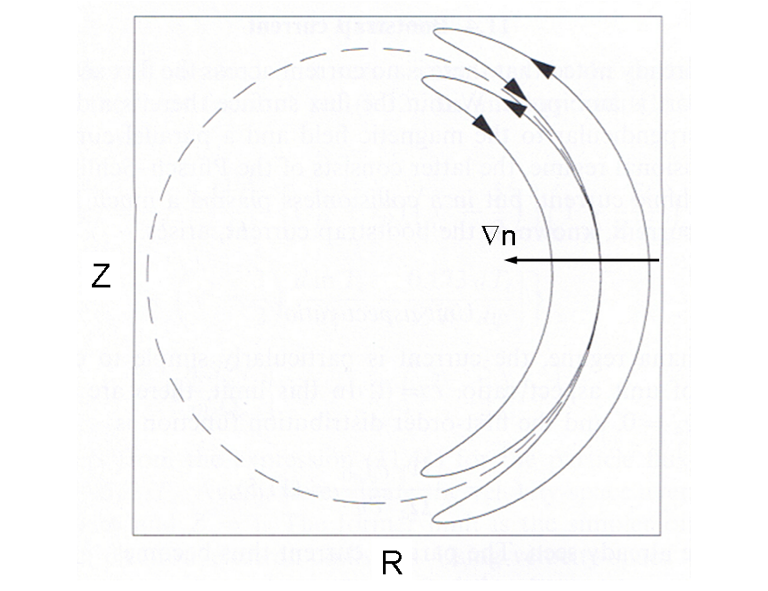
\includegraphics[width=0.50\textwidth]{Fig_bootstrap_1.png}
	\label{fig:bootstrap}
\end{figure}
If the density gradient is directed toward the magnetic axis (as usual), the particle density on the inner trajectory will be larger than that on the outer trajectory. The same comment applies of course for the number of detrapping collisions per time unit, since this number is proportional to the particle density. The net momentum transferred to passing particles due to these detrapping collisions will thus be responsible for a current.

Let us calculate the force (per unit volume) exerted by passing particles due to detrapping:
\[
		\vec{F} = \frac{d\vec{p}}{dt} \simeq \delta n.\nu_{eff}.p_\|
\]
where $\delta n$ is the density difference between the two trapped trajectories at the tangence point, $p_\|$ the particle momentum at this point and $\nu_{eff} = \nu_c/2\epsilon$ the detrapping frequency ($\nu_c$  is the collision frequency). We can express $\delta n$ in the following way:
\[
		\delta n \simeq f_p.\nabla n.\delta_b
\]
where $f_p = \sqrt{2\epsilon}$ is the fraction of trapped particles and $\delta_b = 2q\rho_L/\sqrt{\epsilon}$ is the banana orbit width. The momentum $p_\|$ given to the passing particles when a detrapping collision occurs can be assessed using the trapping condition:
\[
		p_\| = mv_\| \simeq m\sqrt{2\epsilon}v_\perp \simeq m\sqrt{2\epsilon}\sqrt{\frac{2kT}{m}}
\]
Replacing $\rho_L$ and $B_\varphi/B_\theta$ by their usual expressions, we have:
\[
		F \simeq 4\frac{m\nu_c}{eB_\theta}\sqrt{\epsilon}.kT.\nabla n
\]
During these collisions, the passing particles exert a friction force $\nu_c nmv_\|$ of same intensity and opposite sign:
\[
		\nu_c nmv_\| = 4\frac{m\nu_c}{eB_\theta}\sqrt{\epsilon}.kT.\nabla n
\]
from which we deduce the current resulting from detrapping:
\[
		j = env_\| = 4\sqrt{\epsilon} \frac{kT\nabla n}{B_\theta}
\]
This simple calculation allows to exhibit the main dependences of the bootstrap current. We are now going to calculate it in a slightly more precise way.



		\subsection{Calculation of the bootstrap current}
		\label{sub:CalculDuCourantAutoGenere}

An expression of the bootstrap current can be obtained fairly easily using the same equations as those used in the previous section.
The current carried by the plasma is by definition:
\[
		\vec{\jmath} = en \left( \vec{v}_{\varphi,i} - \vec{v}_{\varphi,e} \right)
\]
where $e$ is the proton charge, $n$ is the plasma density (we consider here a plasma of a hydrogenic species (H, D or T) without impurity: $n = n_e = n_i$), subscripts $e$ and $i$ denote electrons and ions respectively, and $v_\phi$ is a toroidal velocity.

Eq. \ref{eq:FluideDuMvt_r} allows to express $j$ as a function of the poloidal velocities:
\begin{equation}
		j = en\frac{B_\varphi}{B_\theta} \left( v_{\theta,i} - v_{\theta,e} \right) - \frac{\nabla p_i + \nabla p_e}{B_\theta}
		\label{eq:densite_courant}
\end{equation}
where $\nabla p_i$ and $\nabla p_e$ are the ion and electron pressure gradients resp. Let us remind that $\nabla p_i + \nabla p_e = \nabla p$.

Subtracting Eq. \ref{eq:FluideDuMvt_par} written for ions from the same equation written for electrons, we obtain an expression of $v_{\theta,i} - v_{\theta,e}$ as a function of the induced electric field $E_{ind}$, of the current density and of the temperature gradients:
\begin{equation}
		v_{\theta,i} - v_{\theta,e} = \left( \frac{1}{\mu_i m_i \nu_i} + \frac{1}{\mu_e m_e \nu_e} \right) e E_{ind} - \left( \frac{\nu_{ie}}{\mu_i \nu_i} + \frac{\nu_{ei}}{\mu_e \nu_e} \right) \left( v_{\|i} - v_{\|e} \right) + \frac{k_i\nabla T_i + k_e\nabla T_e}{e B_\varphi}
		\label{eq:diff_vpol}
\end{equation}

Note that with these new notations, $\nu_i$ and $\nu_e$ are the same as $\nu_{ii}$ et $\nu_{ee}$ defined in Section \ref{subsub:CalculDeLaFréquenceDeCollision}. We thus have:
\begin{eqnarray*}
		\frac{1}{m_i \nu_i} & \simeq & \sqrt{\frac{m_e}{m_i}} \frac{1}{m_e\nu_e}		\\
		\frac{\nu_{ei}}{\nu_e}	&	\simeq	&	1					\\
		\frac{\nu_{ie}}{\nu_i} &	<<	&	1
\end{eqnarray*}
In addition $\mu_e \simeq \mu_i$. this allows us to simplify Eq. \ref{eq:diff_vpol}~:
\[
		v_{\theta,i} - v_{\theta,e} = \frac{e}{\mu_e m_e \nu_e}E_{ind} - \frac{\nu_{ei}}{\mu_e \nu_e} \left( v_{\|i} - v_{\|e} \right) + \frac{k_i\nabla T_i + k_e \nabla T_e}{e B_\varphi},
\]
and replacing in Eq. \ref{eq:densite_courant}~:
\[
		j = \frac{n e^2}{m_e\nu_e \left( 1 + \mu_e\frac{B_\varphi}{B_\theta} \right)} E_{ind} - \frac{1}{1 + \frac{B_\varphi}{\mu_e B_\theta}} \frac{\nabla p - n\left( k_i\nabla T_i + k_e\nabla T_e \right)}{B_\theta}
\]

We recall that $B_\varphi / B_\theta = q / \epsilon$ et $\mu_e B_\theta / B_\varphi = C\sqrt{\epsilon} \ll 1$ (in banana regime), which we use to get a simplified expression of the current density:
\[
		j \simeq \frac{ne^2}{m_e \nu_e}E_{ind} - C\sqrt{\epsilon} \frac{\nabla p - n\left( k_i\nabla T_i + k_e\nabla T_e \right)}{B_\theta}
\]

It can be seen that the first term, proportional to the induced electric field, is the current imposed by the magnetic flux variation in the tokamak coils. The second term is present even without the inductive phenomenon. It exists as soon as there is a pressure gradient in the plasma. It is the self generated current or \textit{bootstrap current}. The factor $\sqrt{\epsilon}$ reminds us that it is due to trapped particles. 


%		\section{Vérifications expérimentales}
%		\label{sec:VerificationsExperimentales}
		
%				\subsection{Courant auto-généré}
				
%				\subsection{Ecrantage de température}
				
%				\subsection{Echecs de la théorie néoclassique}

		\section{Summary of Chapter \ref{chap:TransportCollisionnel}}
		\label{sec:ConclusionNeoclassique}
		
The evaluation of the collision frequency for charged particles of different species and the effect of collisions on the various type of trajectories (passing, trapped) allow to identify three transport regimes: from the weakly collisional to the highly collisional, the banana, plateau and Pfirsch-Schlüter regimes. Electrons are always in the banana regime, light ions are in variable situations depending on the plasma charateristics, and heavy impurities are in the Pfirsch-Schlüter regime. In a more accurate treatment of the problem (which is out of the scope of these notes), all types of trajectories contribute to transport and the total flux of a given species $s$ is of the form:
\[
		\Gamma_s = \Gamma_{cl} + \Gamma_{BP} + \Gamma_{PS}
\]
where $\Gamma_{cl}$ is the classical flux, $\Gamma_{BP}$ is the flux due to collisions involving trapped particles, dominant in the banana and plateau regimes, and $\Gamma_{PS}$ is the flux due to collisions involving  passing particles, dominant in the Pfirsch-Schlüter regime.

We have shown in a particular case that the charged particle flux, whatever the species, is of the diffusive-convective form, which justifies \textit{a posteriori} the assumption done in Chapter \ref{chap:Introduction} for the generic model. The electron convection is directed inward and proportional to the induced electric field. For impurities, we have evidenced the accumulation effect due to the ion density gradient and the temperature screening effect due to the ion temperature gradient. 

In this chapter we have ignored the existence of electromagnetic fluctuations due for instance to the small, short-lived, real charge distribution deviations from the Boltzmann distribution. The effect of these fluctutions is discussed in the next chapter. 

